\section{Implementation of Dynamic Honeycomb Maze}

\subsection{Dynamic Honeycomb Maze Brief}

There are three platform on the hexagon space, one has the mouse placed on it. The is all placed in a room where there is limited space.

\begin{enumerate}
    \item Once the mouse has been place on a platform, there will be two platform that are consecutive to it, that is has the choice to move to. It can either move to one platform or the other. This is entirely the mouse's choice.
    \item Once the mouse has made a choice, and the honeycomb maze has detected this movement, it must move the platforms \textit{without} the animal on it such that they are both consecutive to the (newly positioned) platform with the mouse on it.
    \item This cycle will continue until the mouse has reach the goal required by the experimenter.
\end{enumerate}


Certain abstractions can be made about the platforms robots to help generalise the problem.


Instead of the specific position of the platform with the animal on it, the specific position is abstracted away. 

\begin{figure}
    \centering
    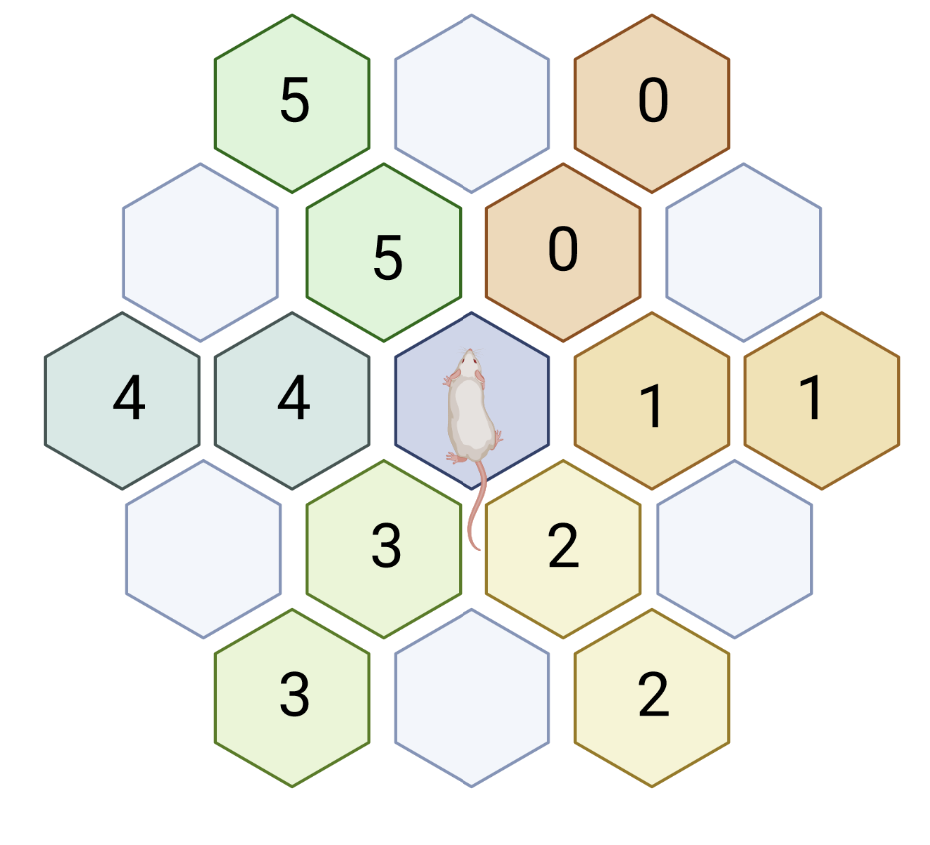
\includegraphics[scale = 0.5 ]{images/relative_position.png}
    \caption{This is a diagramatic representation of the the relative position of a given robot. This is most often applied to the position of the animal robot. 
    \\ Image has been created using 'Biorender' \cite{biorender}}
    \label{fig:relative_position}
\end{figure}

\begin{tabular}{|p{3cm}||p{3cm}|p{3cm}|p{3cm}|}
 \hline
 \multicolumn{4}{|c|}{Table of Relative Position} \\
 \hline
 The axis that is constant & x-axis & y-axis & z-axis \\
 \hline
Relative Position    & 0 \&  3 & 1 \& 4 & 2 \& 5 \\

 \hline
\end{tabular}


The inner an

\begin{figure}
    \centering
    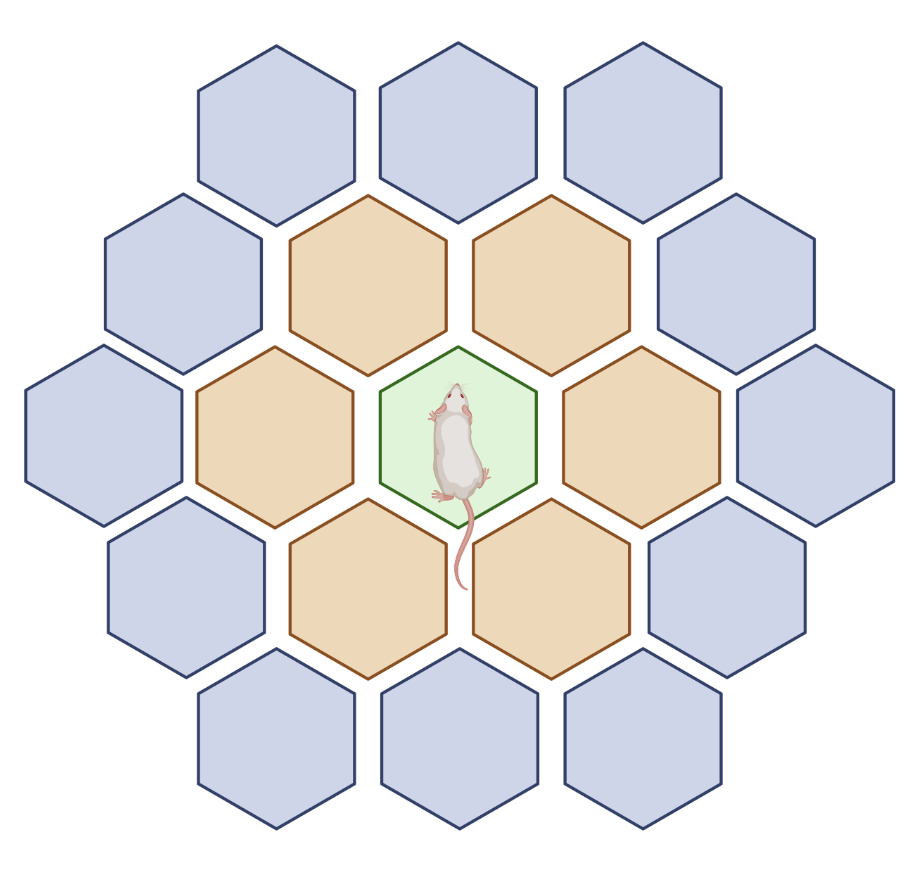
\includegraphics[scale = 0.5 ]{images/outer_rings.png}
    \caption{This figure shows the position of the outer and inner ring, outer ring in orange and inner ring green.\\ This image has been created using 'Biorender' \cite{biorender}}
    \label{fig:my_label}
\end{figure}




\subsection{Maze Class}

This is the class which handles the boundaries of the maze in which the animal and robots can be placed.
It is also important for handling the boundaries of the maze, defining where robots are allowed to move without running out of space in which the robot can move.

\subsubsection{Coordinate system}
Here is where the coordinate system for the 2D hexagonal space was defined:

\begin{figure}
    \centering
    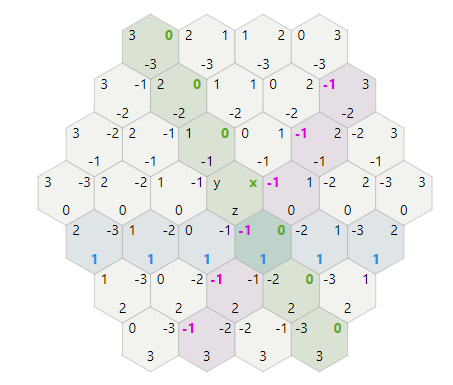
\includegraphics[width=0.7\columnwidth]{images/hexagonal_coordinates.png}
    \caption{The coordinate system used to encode the 2 dimensional space with a 3D coordinate system. The axis have been defined $North-West$ as $x$, $North-East$ as  $y$ and $East-West$ as $z$}.
    \label{Hexagonal grid coordinates}
\end{figure}

Despite the surface on which the platform move around on being flat (and hence 2D), it for the task as hand it is more intuitive to use a 3d coordinate system to encode the space which is being traverse. This is because there are 3 directions in which the platform can move forward: the $North-East$ direction, the $East-West$ direction and the $North-West$ direction.

By convention movement in the $North-East$ direction has been considered to be the $x$ direction, $East-West$ direction to be the $z$ direction and the $North-West$ direction to be considered $y$ direction.
\subsection{Robot Class}

This is the class which deals with the movement of the robot around the maze in which it is places.

Functions defined:
\begin{enumerate}
    \item Defined how to move around the hexagonal grid in a way which is 'legal'
    \item
\end{enumerate}

\subsubsection{Basic moves around the coordinate system}


\begin{algorithm}
\caption{Function for moving around the hexagonal coordinate space}
\require ($x, y, z$)
\end{algorithm}

\subsubsection{Pathfinding around the coordinate space}

Begin able to make the path-finding problem, a graph theory problem allows the problem to be converted to a path-finding problem in graph theory. A a python library is publicly available for the shortest path from two points in a graph network. The library that was used in for the dynamic honeycomb maze is \textit{networkx} \cite{networkx}.

The most advanced = path-finding algorithm supported by networkx is the Dijkstra path-finding algorithm \cite{dijkstra1959pathfinding}. Though this is not as efficient (in most scenarios) as other path-finding algorithms such as the A*  path-finding algorithm \cite{A*_pathfinding}, for the size complexity of network that will be generated for the dynamic honeycomb maze, the Dijkstra path finding algorithm will certainly suffice.



\subsection{Animal Class}

This class is defines the position of the animal, on the robot platform. It is also used for to model the decision making that the animal made when testing the program.


